\chapter{FeedForward Neural Networks}
\label{cha:Neural Network}
\epigraph{
  \hypersetup{linkcolor=bgwhite}
Neural Networks are a set of models inspired by the human brain that can be used to recognize patterns by finding regularities and similarities in data using machine learning data [\cite{patterns}]. The word Neural originates in the
McCulloch-Pitts neuron [\cite{Mcculloch}], a simplified model of the
human neuron as a kind of computing element that could be described in terms of
propositional logic. Just like the
brain, Neural Networks are constructed from small neurons or perceptrons connected with weights. These are made to process and pass on incoming data. The patterns they recognize are numerical, contained in vectors, into which all real-world data, be it images, sound, text, or time series, must be translated first [\cite{Goodfellow-et-al-2016}]. \\

In this chapter, we introduce the basic principles behind a Neural Network.
This will be followed up by the architecture of a FeedForward Neural Network \acrshortrshort{FNN} where the computation proceeds iteratively from one layer of units to the next. This will come in handy for the implementation.  \\
This section’s general introduction to the architecture of FeedForward Neural Networks is mainly based on the books [\cite{Jurafsky2009}] and [\cite{Goodfellow-et-al-2016}]. 



 % Chapter~\ref{cha:anomaly_detection};  
  \hypersetup{linkcolor=linkblue}
}
 

\section{Artificial Neural Networks}
\label{sec:FeedForward}

\begin{figure}
  \centering
  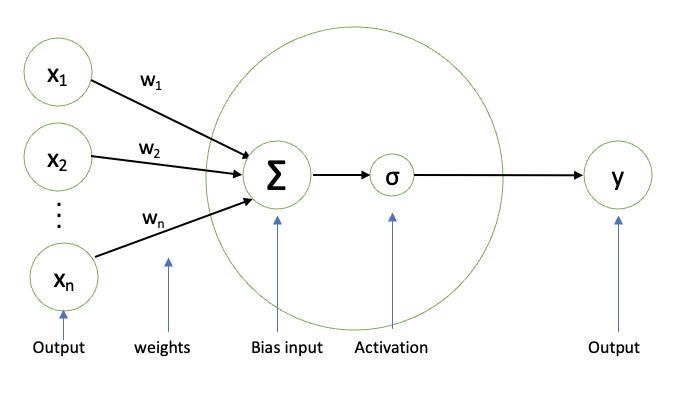
\includegraphics[width=0.7\linewidth]{Pictures/neuron.png}
  \caption{Single neuron model where the neurons $x_i$ takes the n weighted inputs plus a bias. This is an example for a linear case given to the activation function which then outputs an $y$ } 
  \label{fig:perceptron}
\end{figure}

Machine learning is a form of applied statistics focusing on using computers to estimate statistically complicated functions. By having a data set, the goal is to find a function that fits a data set best. One class of modeling is Neural Networks which have been shown to work well. One way to use Neural Network is by applying \acrshortrshort{FNN}.\\
But first consider the mathematical model shown in Figure \ref{fig:perceptron}. This is the simplest example, and the building block of a Neural Network called a single computational unit or a perceptron. A unit takes
a set of real-valued numbers as input, computes them, and produces an output.

More specifically, a Neural unit takes its inputs $x_i$ and their weighted sum $w_i$, which determines the contribution of a given input to the output, with one additional term in the sum called a bias term $b$.
The weighted sum $z$ can be represented as:
\begin{equation}
  \label{eq:ffn_eq}
  z = \sum_i^n w_i x_i + b
\end{equation}
The sum over all the inputs multiplied by their weights can conveniently be represented by a dot product. 
\begin{equation}
  \label{eq:ffn_eq}
  z = w \cdot x + b
\end{equation}

\subsection{Activation functions}
Instead of using a linear function $z$ as the output, Neural units apply a non-linear function $f$ to $z$. This is called an activation function. 
The \emph{feed forward Neural Networks} (FNN) lets information flow through the function being evaluated from x, through the activation function $\sigma$, and finally to the output, $y$. Figure \ref{fig:perceptron} shows a schematic neuron where the unit goes into the activation function and gives the output y.
%shows a simple schematic of a single neuron.
%Since we are only modeling a single unit, the activation for the node is, in fact, the final output of the Network, which we’ll generally call $y$. 
The value $y$ is given by:
\begin{equation}
  \label{eq:activationfunc}
  y = \sigma(z) = \sigma(w\cdot  x + b)
\end{equation}

The bias $b$ measures how easy it is to activate the neuron. Generally, there are a great variety of functions. For this project, we will only discuss the three non-linear functions applied here - the Sigmoid, \acrshort{ReLU}, \acrshort{PReLU} and Softplus.\\

\textbf{Sigmoid}: The sigmoid function, which is shown in Figure~\ref{fig:sigmoid},
\begin{equation}
\label{eq:sigfunc}
  \sigma_{sig} (z) = \frac{1}{1 + e^{-z}},
\end{equation}
takes the real valued number and maps it to a value into the range $[0,1]$ which is useful because the outliers get squashed toward 0 or 1.

\begin{figure}
  \centering
  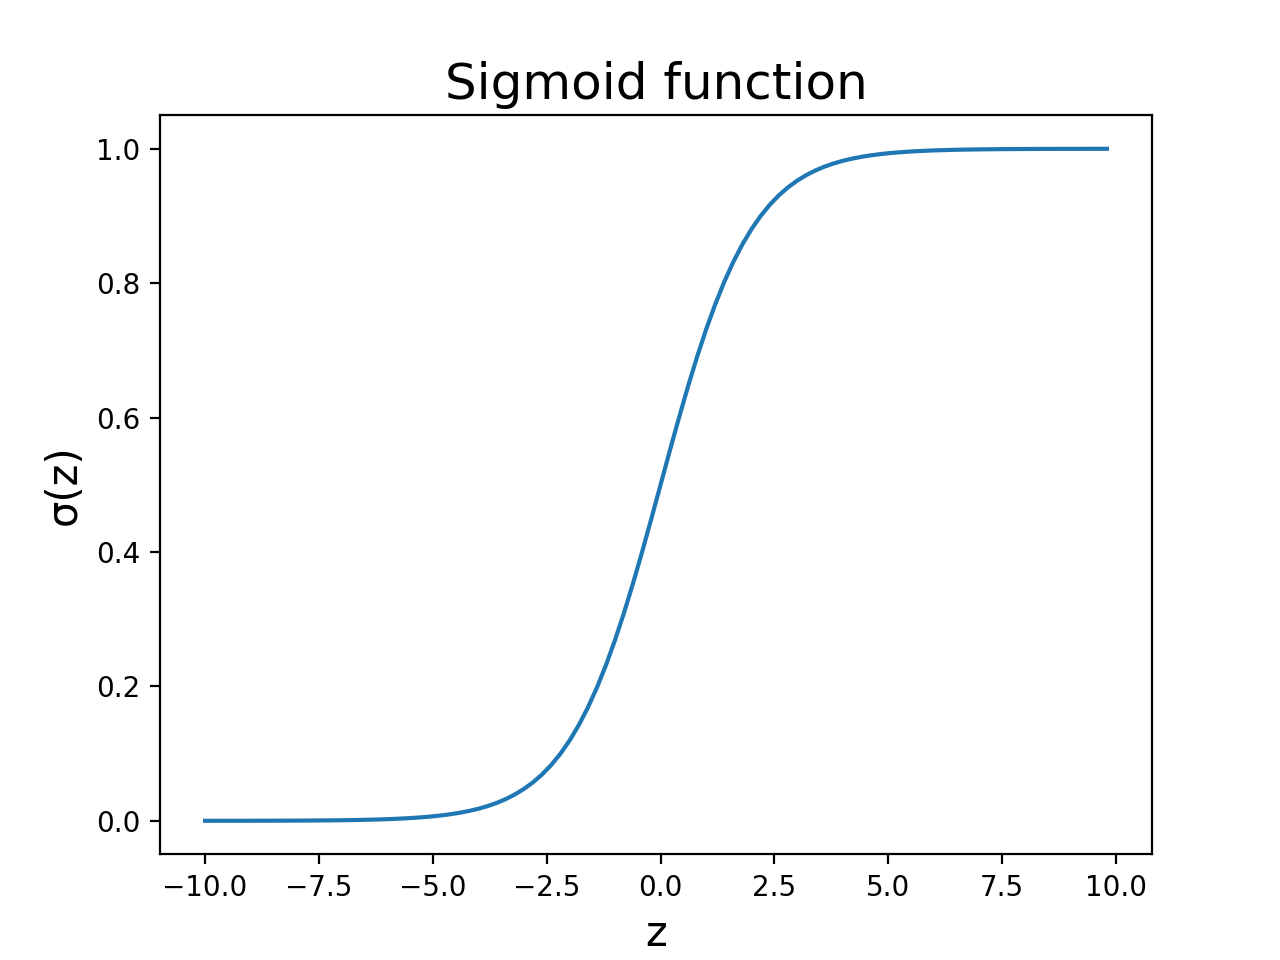
\includegraphics[width=0.5\linewidth]{Pictures/sig.PNG}
  \caption{Sigmoid Function. Frequently used as an activation function in FNN
  The sigmoid function takes a real value and maps it to the range [0,1]}
  \label{fig:sigmoid}
\end{figure}


substituting Eq.\ref{eq:activationfunc} into Eq.\ref{eq:sigfunc} 
gives the output 

\begin{equation}
\label{eq:sig_full}
  y = \sigma_{sig} (w\cdot  x + b) = \frac{1}{1 + exp(-(w\cdot  x + b))},
\end{equation}

\textbf{ReLU}: Rectified Linear Unit is the most commonly used activation function in deep learning models. The function returns 0 if it receives any negative input but returns that value for any positive value  x. So it can be written as

\begin{equation}
%\label{eq:sigfunc},
  y = \sigma_{PReLU} = \begin{cases} x & \text{for x > 0},   \\
        0.01 x & otherwise      %
        \end{cases}
\end{equation}


\textbf{PReLU}: Parametric PReLU (PReLU) makes it a parameter for the Neural Network to figure out itself: $y = \alpha x$ when $x < 0$, where $\alpha$ is a parameter and $x$ is the input. If $x \geq 0$ then $y = x$. 

\begin{equation}
%\label{eq:sigfunc},
  y = \sigma_{PReLU} = \begin{cases} x & \text{for x > 0},   \\
        \alpha x & otherwise      %
        \end{cases}
\end{equation}


PReLU is another popular activation function because it resolves an issue called "the dead neuron problem," which is familiar with the ReLU function. This problem occurs when inputs approach zero or are negative, which will make the gradient of the ReLU function
zero [\cite{QingJie_2017}]. This implies that with poor initialization, where most neurons have negative output, these
neurons will have no incentive to adjust their weights. Hence the Network will have limited ability to "learn.” PRelu addresses this issue, given that it doesn’t have zero-slope parts.\\


\textbf{SoftPlus}: Finally, the softplus function is a smooth approximation to the PReLU activation function and is sometimes used in the Neural Networks in place of PReLU. It is closely related to the sigmoid function. In particular, when $x \to$ −$\infty $, the two functions become identical.

\begin{equation}
\label{eq:softfunc}
 \sigma_{soft}= \log\left(1+\exp{x}\right),
\end{equation}

However, these activation functions have different properties, making them useful for different Network architectures. For example, the \acrshortrshort{ReLU} function has beneficial properties. Networks trained with the rectifier function almost completely avoid the problem of vanishing gradients, as the gradients remain proportional to the node activations [\cite{Goodfellow-et-al-2016}]. Contrary to the sigmoid function, containing exceptionally high values of $z$ result in values   of $y$ that are saturated, i.e.,
Extremely close to 1, which causes problems for learning [\cite{Jurafsky2009}]. Rectifiers don’t have this problem since the output of values close to 1 also approaches 1 in an excellent gentle linear way.

\subsection{The XOR problem}
\label{sec:xor_problem}
When sending data to a unit, it goes through the activation function, which reduces the sum of the input values to a 1 or 0 value, or at least a value very close to. If we consider the task of computing elementary logical functions of two inputs, like AND, OR, and XOR, we get the truth tables, as shown in Figure \ref{fig:truthtables}

\begin{figure}
  \centering
  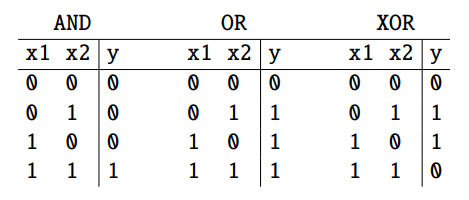
\includegraphics[width=0.5\linewidth]{Pictures/truthtable.PNG}
  \caption{Truth tables of elementary logical functions of two inputs for AND, OR and XOR. The XOR gives the output 1 if the inputs are different from each other and 0 if they are the same }
  \label{fig:truthtables}
\end{figure}

On the surface, this appears to be a simple problem. However, as shown by Minsky and Papert in 1969 [\cite{minsky69perceptrons}], this becomes an issue for a Neural Network that is only based on a single perceptron. The difference is that a perceptron is purely linear, and a unit is non-linear. If we look at a two-dimensional problem for the different truth-tables in Figure \ref{fig:xorgraph}, we see the possible logical inputs (00, 01, 10, and 11) and the line drawn
by one possible set of parameters for an AND and an OR classifier. 
If we look at the AND example we see, that when $x1=1$ and $x2=1$ then $y=1$ and in all other cases, it is 0, so if you wanted to separate all the ones from the zeros by drawing a single line, you would draw the line as shown in the graph.

\begin{figure}[h]
  \centering
  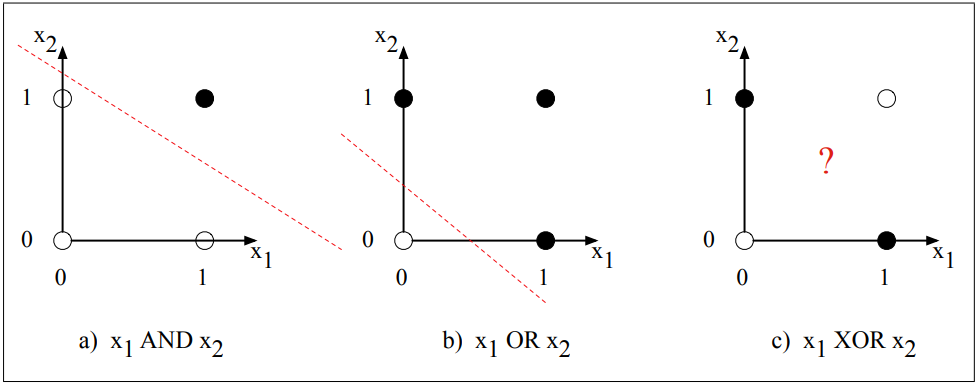
\includegraphics[width=0.7\linewidth]{Pictures/XORgraph.PNG}
  \caption{Truth-tables of elementary logical functions of two inputs for AND, OR and XOR [\cite{Jurafsky2009}]}
  \label{fig:xorgraph}
\end{figure}

A single line can separate this class. They are linearly separable patterns, meaning classes with an n-dimensional vector can be divided with a single decision surface.

That is how the perceptron works; it draws a boundary to separate the binary values. When the perceptron is trained, the value of the weights will be adjusted to form the line shown. Since the perceptron's output is a linear function, the two classes must be linearly separable for the perceptron Network to function correctly. 

Let’s see what happens with XOR problem that gives $y=1$ if $x_1\neq x_2 $ and  $y=0$ otherwise.
Notice that there is simply no way to draw a line that separates the positive cases of XOR (01 and 10) from the negative points (00 and 11). Hence, we conclude that XOR is not a linearly separable function.
Instead, we will have to draw multiple lines and thus require various perceptrons. In n-dimension, if you can draw a hyperplane to separate the binary values, you can use perceptrons to solve that problem.



\section{FeedForward Neural Network}
Having provided the necessary background knowledge behind units/perceptrons and how they work, next, we will need to elaborate on the functioning of the \textbf{FeedForward Neural Network or FNN}. A FeedForward Network consists of multiple layers in which the units are only connected in one way and
often applied to classification tasks, such as the recognition of a certain
shape in an image. There are three layers: the input, hidden, and output layers.  However, the characteristic and core of a \acrshortrshort{FNN} is the hidden layer, which consists of units described in \ref{eq:activationfunc}. The output of each layer is passed to teams in the hidden layer, which sums over all the input units until the final layer gives the final output. Figure \ref{fig:fnn_layers} shows an FNN where the input layer represents the data that is fed into the Network, followed by one or more hidden layers and an output layer.

We can think of a fully-connected Network as a function $F$ : $\mathbb{R}^n \to \mathbb{R}^m$ that maps the input $(x_1, .., x_n)$ to the output $(y_1, .., y_m)$ We
are now considering a structure of numerous neuron ordered in different layers. Therefore, $F$ can be split into a chain of simpler functions $f^{(i)}$, where  $f^{(i)}$ correspond to activation/output of the neurons in the i'th layer.

\begin{equation}
    F(x) = f^{(out)}(..f^{(i)}(..f^{(1)}(x)..)..),
\end{equation}

Where the first layer after the input layer is represented by $f^{(1)}$ and the final layer as $f^{(out)}$, the input layer is usually not counted when enumerating layers, but we call it the 0'th layer.

In a Neural Network, we only know the
input and the output from the final layer. The activation  $f^{(i)}$ of the layers in between is not shown, which is why
they are called hidden layers. A network consisting of more than one hidden layer is called \emph{deep Neural Network}, where we define the model depth as the number of hidden layers in the Network, thus, not counting the input and output layer. 
It is common for hidden layers to be much larger than
the input and output layer in deep Neural Networks because having larger dimensions give the best prediction [\cite{Goodfellow-et-al-2016}].  The number of weights for deep
Therefore, networks become approximately proportional to the square of the count of
nodes per layer in these largely hidden layers. Instead, we can think of layers as we described the neurons. Now just with a bias $b$ as a vector and the weight as a matrix $W$, consisting
of the combination of the weight vector $w_i$ and bias $b_i$ for each unit $i$. From a visual point of view as illustrated in Figure \ref{fig:fnn_layers}, we can represent each element of matrix $W$ as $W_{ji}$ where it connects the   $i$th input $x_i$ unit to the $j$th hidden unit $h_j$. By representing it with a single weight matrix $W$, the output of the hidden layer $h$ is thus:

\begin{equation}
  h = \sigma(W x + b)
  \label{eq:hidden_layer}
\end{equation}

where $\sigma$ is applied to a vector elementwise, so $\sigma[z_1,z_2,z_3] = [\sigma z_1,\sigma z_2, \sigma z_3]$.

The dimensionalities of these vectors
and matrices are enumerated as $n_0, n_1$ and $n_2$ for respectively the input, hidden and output layer. Here $x \in \mathbb{R}^{n_0}$, $h \in \mathbb{R}^{n_1}$ and $b \in \mathbb{R}^{n_1}$, since each hidden layer can take a different bias. The weight matrix therefor has dimensionality $W \in \mathbb{R}^{n_1 x n_0}$.

The matrix multiplication from equation~\ref{eq:hidden_layer} is thus:

\begin{equation}
    \begin{split}
  h & = \sigma \left(\sum^{n_0}_{i =1}  W_{ji} * x_i  + b_j\right) \\
  &= f^{(i)} = \sigma (W^{(i)} *  f^{(i-1)}  + b^{(i)})
    \end{split}
\end{equation}

\begin{figure}
  \centering
  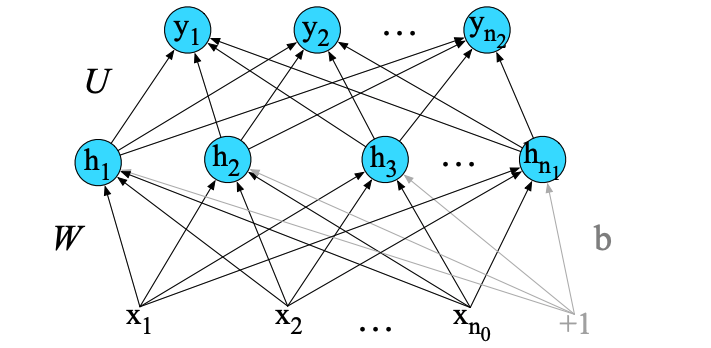
\includegraphics[width=0.7\linewidth]{Pictures/fnn_layers.png}
  \caption{A simple FeedForward Network, with one input layer (not counted as layer), hidden layer and one output layer [\cite{Jurafsky2009}]. }
  \label{fig:fnn_layers}
\end{figure}



where $f^{(i-1)}$ is the output from the $(i-1)^{th}$ layer.
Like the hidden layer, the output layer also has a weight matrix $U$ and sometimes a bias, but we will look at a simple example without the bias for simplicity’s sake.
The weight matrix for the output layer is multiplied by its input vector from the layer before, which is the hidden layer $h$, to produce the intermediate output z.

The output of the hidden layer $h$ is thus:
\begin{equation}
  z = U h
\end{equation}

Since z is a vector of real-valued numbers and needs a classification of probabilities, we can use a normalization function such as the softmax to get a probability distribution.
The output of the hidden layer $h$ is thus:
\begin{equation}
  y = \text{softmax}(z)
\end{equation}

In this way, the layers in FNNs can model arbitrary functions and separate data sets that are not linearly separable. This linearity is only broken by the activation function contained in the hidden layers, which act as a non-linear transform that distorts the input. It is done in such a way that its classes become linearly separable by the output layer as explained in the \ref{sec:xor_problem}.

\iffalse
\begin{figure}
  \centering
  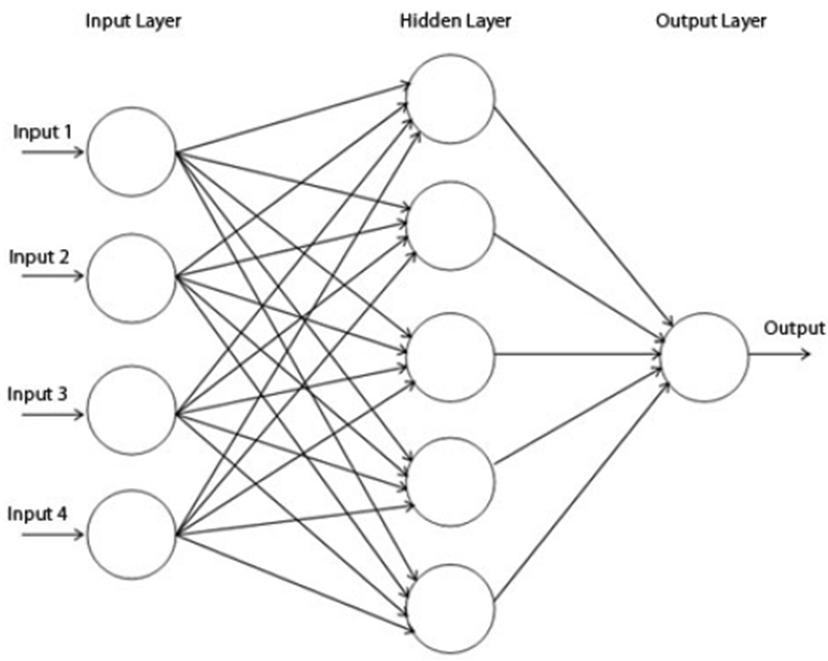
\includegraphics[width=0.5\linewidth]{Pictures/fnn.png}
  \caption{\hl{NEED PICTURE OF MY FNN REAL AMOUNT OF LAYERS Fully connected FeedForward Neural Network with a single hidden layer and one output neuron.}}
  \label{fig:fnn}
\end{figure}
\fi

\iffalse
represented as a chain of a function per layer in the model as e.g. $f(x)=f^{(3)}(f^{(2)}(f^{(1(x)})))$ which is a representation for a model with
two hidden layers as shown in figure \ref{fig:fnn_la}.  Here $f^{(1)}$ and $f^{(2)}$ are the functions of the
first and second hidden layer respectively. The outermost function $f^{(3)}$ is the function for the output layer. We can describe the first layer as $x_i = h_i^{(0)}$, such that the first layer is the 0'th. 
\fi

\subsection{Universal Approximation Theorem}
One of the unique properties of neural networks is that they can compute any function at all and can be approximated by any Borel measurable function [\cite{hornik1991approximation}]. A more straightforward explanation is that the Universal Approximation Theorem states that a Neural Network with one hidden layer can approximate any continuous function for inputs within a finite-dimensional space to another with any desired non-zero amount of error, provided that the Network is given enough hidden units. However, it does not state how large this Network needs to solve the given problem, so this is still done by trial and error methods.



\section{Training of a Neural Network}
feedforward neural networks are mainly used for supervised learning where the data to be learned is not sequential nor time-dependent. This implies that we know the correct output $y$ for each observation $x$. What the system produces is an estimate of $\hat{y}$ (the true y).
The goal of the machine learning approach is to find a weight and bias configuration for each layer that captures the quintessence of the presented data set, that make the estimate of y for each training
observation as close as possible to $\hat{y}$.
Currently, the Network is very much dependent on the training data-set. It should ideally include all kinds of combinations of possible inputs. This can be difficult to do in practice and the available data-sets are therefore typically split randomly into three
categories: \emph{training}, \emph{validation}, and \emph{test} set.\\

The \textbf{training set} is the actual data set that we use to train the model (weights and biases in the case of a Neural Network). The model sees and learns from this data. 
We will need a loss function that models the distance between the system output and the expected output.
The commonly used technique to train the model is by some variation of Gradient Descent \acrshortrshort{GD}. GD algorithms try to minimize a particular loss or cost function with respect to a given weight configuration.
The \textbf{validation set} is used to provide an unbiased evaluation if a model fits on the training data-set. This tells how to change the Network's weights and biases overall behavior, also known as tuning hyperparameters. The evaluation becomes more biased as a skill on the validation data-set is incorporated into the structure of the model. To reduce the risk of overfitting, the optimization
should be stopped as soon as the error on the validation set is not decreasing
any more. 
Generally, over-fitting occurs when a model learns the training data set too well, performing smoothly on the training data set but can not seem to work on a different sample [\cite{Kriesel2007NeuralNetworks}] 
This is one of the other methods applied in machine learning to achieve a generalization over previously unseen data points. Because the information of the validation set is leaking into the Network via the early stopping criterion, a third data set is needed to evaluate the actual performance and generalization of the Network. This third set is called the \textbf{test set}.
The test set is a benchmark used to evaluate the model and is only used once a model is thoroughly trained. However, the focus in this project is to accelerate an already trained model and does therefore not have to be taught any further.


\iffalse
\hl{FNNs contain many good advantages of training data. However, there are also some disadvantages. Backpropagation algorithms, which is this method for calculating the gradient of the error function concerning the Neural Network's weights, typically need vast amounts of data to train the Network. When using gradient descent, the steps have to be small enough not to jump over the desired minima,
which leads to very long training times. Data training can lead to unexplained results if it does not
properly represent the possible parameter space. It will then be more difficult to interpret how the Network came to a specific result, as the weight matrices do not represent traceable reasoning or logic. }
\fi

\begin{figure}
  \centering
  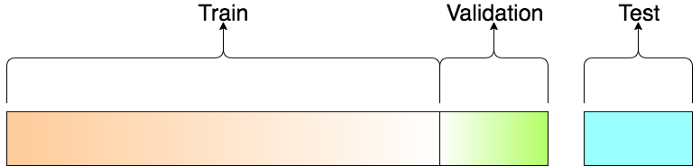
\includegraphics[width=0.5\linewidth]{Pictures/splitdata.png}
  \caption{All data used for training a ML model, split up in a \emph{training}, \emph{validation}, and \emph{test} set}
  \label{fig:fnn}
\end{figure}

\iffalse
\subsubsection{Loss function}

The most commonly used loss function in Neural Networks is the \textbf{cross-entropy loss} when optimizing classification models. We will use this loss function when training our model. It tells us how good our Neural Network is for a specific task.
Cross-entropy loss measures the performance of a classification model whose output is a probability value between 0 and 1. Cross-entropy loss increases as the predicted probability diverge from the actual label, depending on the classification and the activation function used for the output layer.
 The loss function is given by:

\begin{equation}
L(y,\hat{y}) = \frac{}{}
\end{equation}




\section{Gradient descent}
\label{sec:GD}
\fi

\newpage

\section{Our FNN model}
Now that we have the background, we can start looking at the provided model, which is written in Python using the \texttt{Pytorch} library. 
\subsection{Pytorch}

PyTorch is an open-source machine learning library based on the Torch library used for applications such as computer vision and NLP [\cite{pybook}]. It is an open-source library maintained mainly through Facebook’s AI research group.
Unlike other popular frameworks like TensorFlow, which uses static computation graphs, PyTorch uses dynamic computation, allowing greater flexibility in building complex architectures. It uses core Python concepts like classes, structures, and conditional loops, which are easier to understand intuitively. This makes it a lot simpler than other frameworks, such as TensorFlow that incorporates their programming style.
To understand how the model is built, we will quickly go through some features o the PyTorch used in the given script. \\


\subsection{Torch}
PyTorch defines a class called \texttt{Torch.Tensor} which contains data structures for multi-dimensional tensors and mathematical operations. It stores and operates on homogeneous multidimensional rectangular arrays of numbers. "PyTorch Tensors are similar to NumPy Arrays but can also be operated on a CUDA-capable Nvidia GPU.
Additionally, it provides many utilities for efficient serializing of Tensors and arbitrary types, and other valuable utilities" [\cite{py}].



\subsection{Torch.nn}
The \texttt{Torch. nn} PyTorch auto grad makes it easy to define computational graphs and take gradients, but raw auto grad can be a bit too low-level for defining complex Neural Networks. This is where the nn module comes in handy. This model uses \texttt{nn.module} and \texttt{nn.parameter}. The \texttt{nn.module} performs operations on tensors. Modules are implemented as subclasses of the \texttt{torch.nn.module} class. All modules are callable and can be composed together to create complex functions.
the \texttt{nn.parameter} is a tensor that sub-classes the Variable class.
The difference between a variable and a parameter comes in when associated with a module. When a parameter is associated with a module as a model attribute, it automatically gets added to the parameter list and can be accessed using the 'parameters' iterator. \\

The provided FNN model takes in an input $x$ and a target $y$. The weights and data are generated randomly.
I started with a minimal data set to understand each process going through the model to understand all the calculations. This FeedForward Neural Network model consists of two layers shown in Listing \ref{lst:layers}. 
This model is a part of a more extensive pipeline where the models are trained to recognize features that indicate an upcoming increase or decrease in the market pricing and bid accordingly.
Deep Learning methods, while known in general to be highly successful in terms of accuracy, also carry a curse of heavy computations with them. Therefore, we will implement it with SME in the next section and test if we can keep the accuracy and accelerate the inference.


\iffalse
\begin{listing}
  \inputminted{python}{codesnippets/forward.py}
  \caption{Forward function calling all layers used in the FeedForward model}
  \label{lst:forward}
\end{listing}
\fi

\begin{listing}
  \inputminted{python}{codesnippets/fnn.py}
  \caption{The different layers and functions used in the FNN Network}
  \label{lst:layers}
\end{listing}





